\documentclass{beamer}
\usepackage{algorithmic}

\title{KeyChain Extension and Integration}
\subtitle{Presentation}
\author[Braden, Dickhaus, Puodzius]{Kjell Braden, Marvin Dickhaus, Cassius Puodzius}
\institute{Fachbereich Informatik \\ TU Darmstadt}
\date{March 27, 2013}

\usetheme{Berkeley}
\usecolortheme{dove}

\begin{document}
\begin{frame}
	\titlepage
\end{frame}
\begin{frame}
	\tableofcontents
\end{frame}

\section{Motivation}
	\begin{frame}
		\tableofcontents[currentsection]
	\end{frame}
	\begin{frame}
	\frametitle{Motivation}
	\begin{itemize}
		\item KeyChain is poorly used in current Android Versions
		\item Lack of integration between key access and its use
		\item Broader acceptance of encryption % What does it mean?
	\end{itemize}
	Goals:
	\begin{itemize}
		\item Improve secure storage and authorization handling for keys
		\item Support easy use of cryptographic functions for apps
	\end{itemize}	
	\end{frame}

\section{Requirements}
	\begin{frame}
		\tableofcontents[currentsection]
	\end{frame}
	\begin{frame}
	% this should be things the api has to fulfil/provide, not technical requirements!
	\frametitle{Requirements}
		Apps should be able to...
		\begin{itemize}
			\item run common crypto operations without accessing keys directly
			\item generate, store and export symmetric keys
			\item store and export public keys
			\item run key agreement protocols 
			\begin{itemize}
				\item store the key agreement parameters in the KeyChain
				\item automatically derive and store the shared secret key in the KeyChain
			\end{itemize}
		\end{itemize}
	\end{frame}

\section{Implementation Issues}
	\begin{frame}
		\tableofcontents[currentsection]
	\end{frame}
	\begin{frame}
		\frametitle{Existing Android API}

		\begin{block}{Java Cryptography Architecture (JCA)}
		\begin{itemize}
			\item offers interfaces for SecretKey/PublicKey/PrivateKey
			\item offers factories for ciphers, signature schemes etc. to work on the corresponding implementation of keys
		\end{itemize}
		\end{block}

		\begin{block}{native (C++) keystore daemon}
		\begin{itemize}
			\item stores key material encrypted using phone lock passphrase, pin or pattern
			\item offers an OpenSSL engine for loading JCA Key objects from the store without exposing the key material itself, but...
				\begin{itemize}
					\item there is no real access control
					\item only RSA keys are supported
					\item attempting to use the keys for anything causes a SIGSEGV in dalvik {\tt :-(}
				\end{itemize}
		\end{itemize}
		\end{block}
	\end{frame}
\section{Implementation Details}
	\begin{frame}
		\tableofcontents[currentsection]
	\end{frame}
	\begin{frame}
		\frametitle{Overview}
		\begin{itemize}
			\item a system app for key management, such as
				\begin{itemize}
					\item key generation
					\item import/export/deletion of key pairs
					\item granting key access
				\end{itemize}
			\item a public API which allows
				\begin{itemize}
					\item encryption / decryption
					\item authentication (signature/MAC) / verification
					\item generation / import of symmetric keys
					\item key agreement protocols
				\end{itemize}
		\end{itemize}
	\end{frame}

	\begin{frame}
		\frametitle{Key Identification}
		\begin{itemize}
			\item each key is referenced by a unique string alias
			\item keys can be assigned to contacts using the {\em Key Management} app
			\item each assignment has a {\em key usage type identifier}
				\begin{itemize}
					\item arbitrary string token (application defined)
					\item apps can request a key with a given type for a given contact
					\item this way the user can easily choose which key to use for which app, and replace keys once they are obsoleted
				\end{itemize}
		\end{itemize}
	\end{frame}

	\begin{frame}
		\frametitle{API usage}
		\begin{itemize}
			\item API calls are forwarded using binder IPC to the {\em keychain} system app
			\item system app checks if the calling app is allowed to use the key
			\item system app may present the user with a dialog to authorize the access
			\item if authorized, the system app processes the request and sends the result back to the caller
		\end{itemize}
	\end{frame}

\section{Encrypted SMS}
	\begin{frame}
		\tableofcontents[currentsection]
	\end{frame}
	\begin{frame}
	\frametitle{Considerations}
		\begin{itemize}
			\item Separate UI for sending
			\item Lookup of keys (key usage type)
			\item Storage of SMS %in the global SMS content provider
			\item Recognize encrypted messages
			\item Keep it as simple as possible %user doesn't have to differ from it's known android behavior.
		\end{itemize}
	\end{frame}
	\begin{frame}
	\frametitle{Sending and Receiving}
		\begin{block}{Sending}
			\begin{itemize}
				\item Select contact
				\item Encrypt composed message
				\item Send Base64-encoded message via SMS
				\item Store copy of plain message locally
			\end{itemize}
		\end{block}
		\begin{block}{Receiving}
			\begin{itemize}
				\item Capture {\tt SMS\_RECEIVED} broadcast
				\item Recognizing encrypted SMS
			\end{itemize}
		\end{block}
	\end{frame}
	\begin{frame}
		\frametitle{Receiving Workflow}%Can be ignored if there is no time left.
		\begin{algorithmic}
			\REQUIRE {all message parts have been received and the full message is reassembled}
			%\IF{the SMS is encrypted\footnote{determined by @-char at the beginning and end}}
			%\IF{sender has a key assigned}
			%	\STATE {\tt abort broadcast}
			%	\STATE {\tt decrypt SMS}
			%	\STATE {\tt store decrypted SMS in the conversation log}
			%\ENDIF
			%\ENDIF
		\end{algorithmic}
		\begin{figure}[h]
			\centering
			\includegraphics[width=17em]{sms_receive}
			\caption{Receiving workflow}
			\label{fig:receive}
		\end{figure}
	\end{frame}

	
\section{Trivia}
	\begin{frame}
		\tableofcontents[currentsection]
	\end{frame}
	\begin{frame}
	\frametitle{Trivia}
		%Amount spend by Kjell generating Images 10, 20, 40 hours?
		\begin{itemize}
			\item time spent building full images: approx. 80 hours
			\item RSA 1024-bit key generation
				\begin{itemize}
					\item regular MIPS emulator image: 10 minutes
					\item x86 emulator image using VT-x/AMD-V: less than 5 seconds
				\end{itemize}
		\end{itemize}
	\end{frame}

\end{document}
